\documentclass[../main/main.tex]{subfiles}

\begin{document}

\newpage

\section{Design}
\subsection{System Architecture}
In this section, I will lay out the overall logic, and an overview of the steps involved in running my program. By decomposing the program into individual abstracted stages, I can focus on the workings and functionality of each section individually, which makes documenting and coding each section easier.I have also included a flowchart to illustrate the logic of each screen of the program.

I will also create an abstracted GUI prototype in order to showcase the general functionality of the user experience, while acting as a reference for further stages of graphical development. It will consist of individually drawn screens for each stage of the program, as shown in the top-level overview. The elements and layout of each screen are also documented below.

The following is a top-level overview of the logic of the program:

\begin{figure}[ht!]
    \centering
    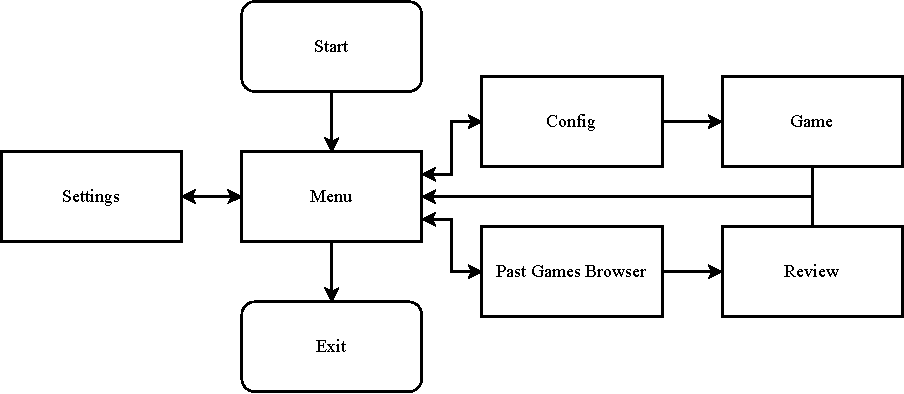
\includegraphics[width=\columnwidth]{../design/assets/top_level_overview_flowchart.pdf}
    \caption{Flowchart for Program Overview}
    \label{fig:program-overview-flowchart}
\end{figure}

\subsubsection{Main Menu}
\begin{figure}[ht!]
    \centering
    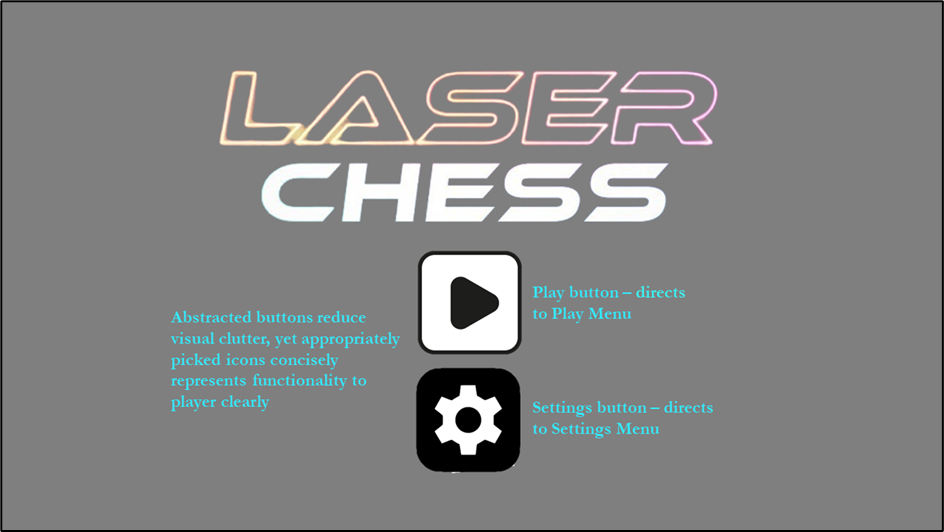
\includegraphics[width=0.8\columnwidth]{../design/assets/menu_gui.png}
    \caption{Main Menu screen prototype}
    \label{fig:menu-gui}
\end{figure}

The main menu will be the first screen to be displayed, providing access to different stages of the game. The GUI should be simple yet effective, containing clearly-labelled buttons for the user to navigate to different parts of the game.

\subsubsection{Settings}
\begin{figure}[ht!]
    \centering
    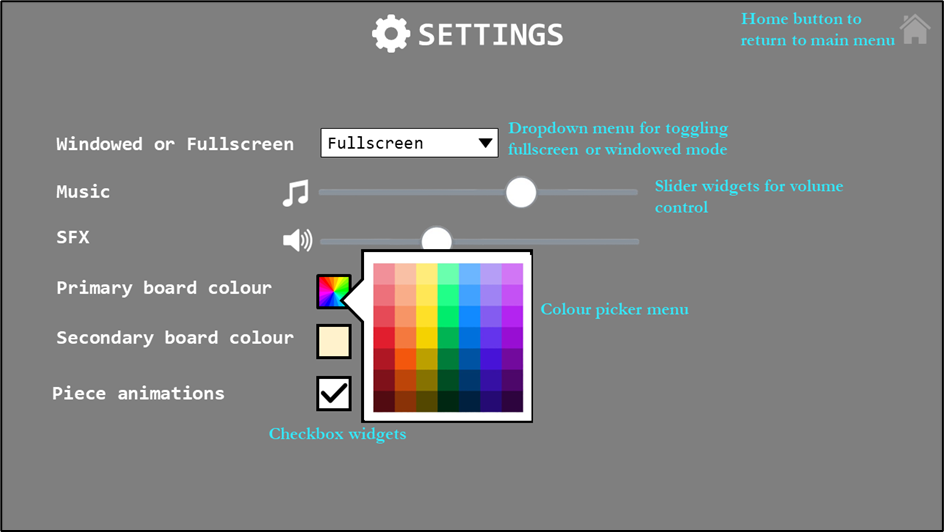
\includegraphics[width=0.8\columnwidth]{../design/assets/settings_gui.png}
    \caption{Settings screen prototype}
    \label{fig:settings-gui}
\end{figure}

The settings menu allows for the user to customise settings related to the program as a whole. The settings will be changed via GUI elements such as buttons and sliders, offering the ability to customize display mode, volume, board colour etc. Changes to settings will be stored in an intermediate code class, then stored externally into a JSON file. Game settings will instead be changed in the Config screen.

The setting screen should provide a user-friendly interface for changing the program settings intuitively; I have therefore selected appropriate GUI widgets for each setting:

\begin{itemize}
\item Windowed or Fullscreen - Drop-down list for selecting between pre-defined options
\item Music and SFX - Slider for selecting audio volume, a continuous value
\item Board colour - Colour grid for the provision of multiple pre-selected colours
\item Piece animation - Checkbox for toggling between on or off
\end{itemize}

Additionally, each screen is provided with a home button icon on the top right (except the main menu), as a shortcut to return to the main menu.

\begin{figure}[ht!]
    \centering
    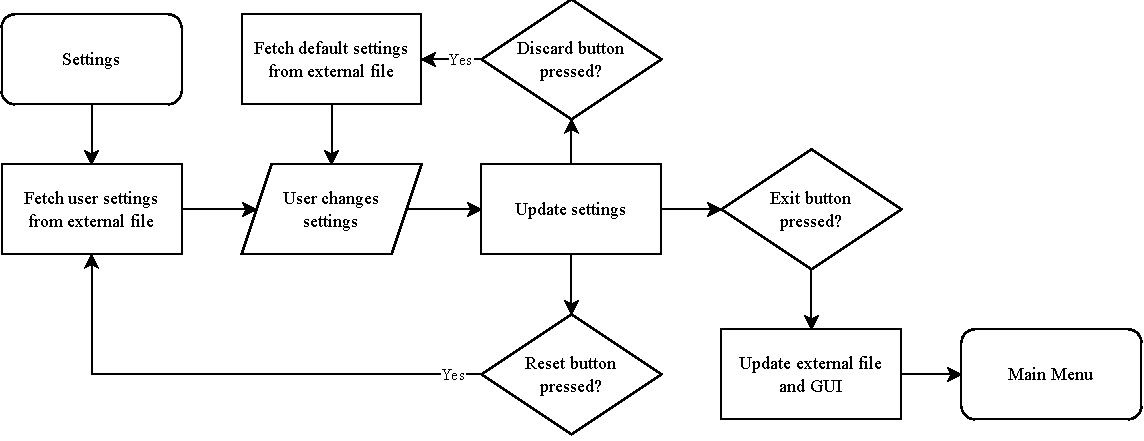
\includegraphics[width=\columnwidth]{../design/assets/settings_flowchart.pdf}
    \caption{Flowchart for Settings}
    \label{fig:settings-flowchart}
\end{figure}

\subsubsection{Past Games Browser}
\begin{figure}[ht!]
    \centering
    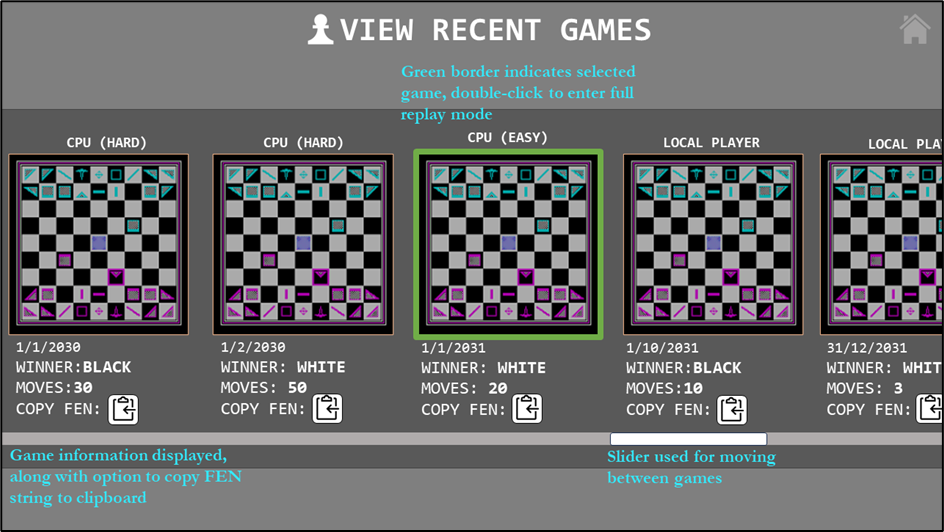
\includegraphics[width=0.8\columnwidth]{../design/assets/browser_gui.png}
    \caption{Browser screen prototype}
    \label{fig:browser-gui}
\end{figure}

The Past Games Browser menu displays a list of previously played games to be replayed. When selecting a game, the replay will render out the saved FEN string into a board position identical to the one played previously, except the user is limited to replaying back and forth between recorded moves. The menu also offers the functionality of sorting games in terms of time, game length etc.

For the GUI, previous games will be displayed on a strip, scrolled through by a horizontal slider. Information about the game will be displayed for each instance, along with the option to copy the FEN string to be stored locally or to be entered into the Review screen. When choosing a past game, a green border will appear to show the current selection, and double clicking enters the user into the full replay mode.
While replaying the game, the GUI will appear identical to an actual game. However, the user will be limited to scrolling throughout the moves via the left and right arrow keys.

\begin{figure}[ht!]
    \centering
    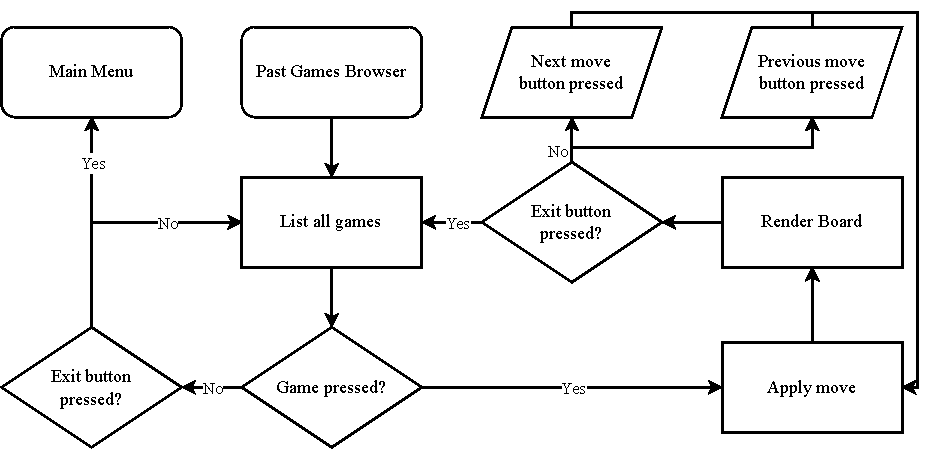
\includegraphics[width=\columnwidth]{../design/assets/browser_flowchart.pdf}
    \caption{Flowchart for Browser}
    \label{fig:browser-flowchart}
\end{figure}

\subsubsection{Config}
\begin{figure}[ht!]
    \centering
    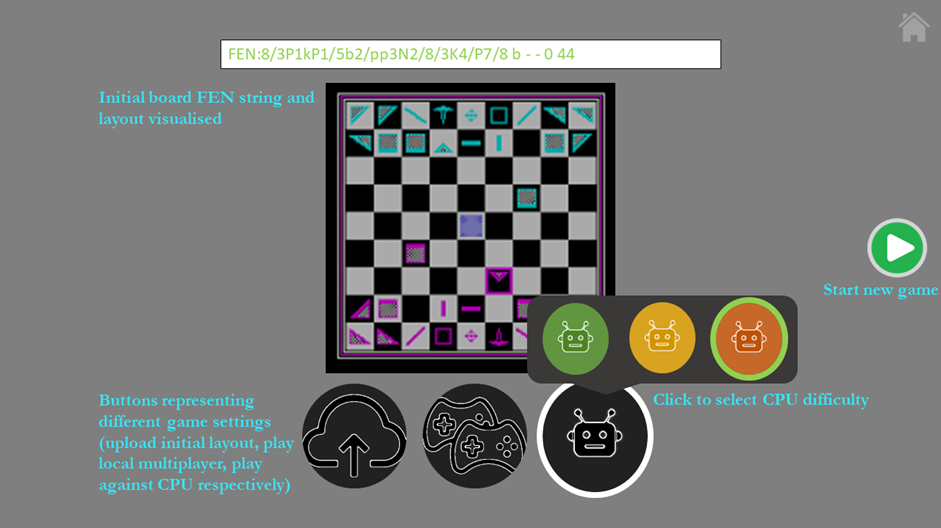
\includegraphics[width=0.8\columnwidth]{../design/assets/config_gui.png}
    \caption{Config screen prototype}
    \label{fig:config-gui}
\end{figure}

The config screen comes prior to the actual gameplay screen. Here, the player will be able to change game settings such as toggling the CPU player, time duration, playing as white or black etc.

The config menu is loaded with the default starting position. However, players may enter their own FEN string as an initial position, with the central board updating responsively to give a visual representation of the layout. Players are presented with the additional options to play against a friend, or against a CPU, which displays a drop-down list when pressed to select the CPU difficulty.

\begin{figure}[ht!]
    \centering
    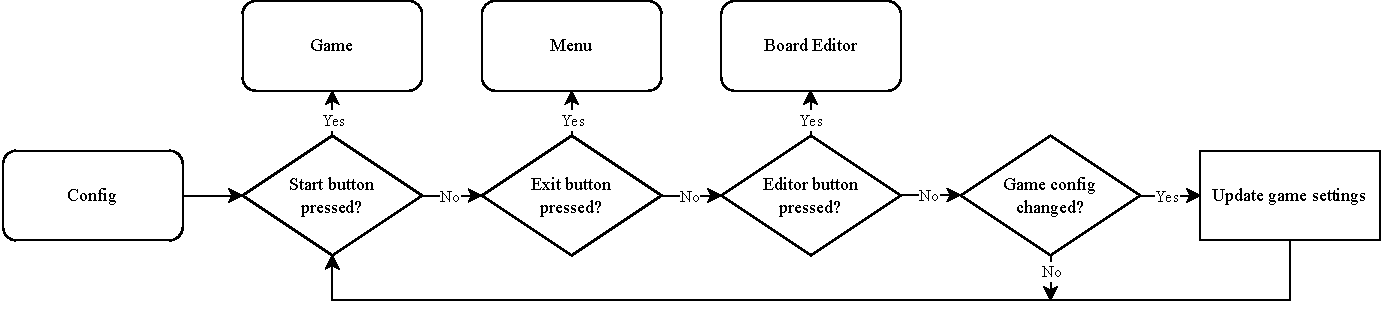
\includegraphics[width=\columnwidth]{../design/assets/config_flowchart.pdf}
    \caption{Flowchart for Config}
    \label{fig:config-flowchart}
\end{figure}

\subsubsection{Game}
\begin{figure}[ht!]
    \centering
    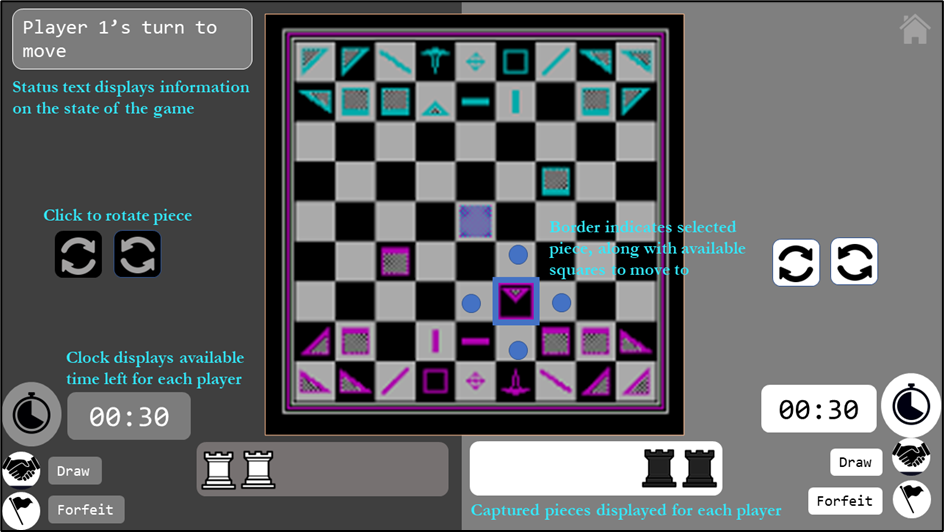
\includegraphics[width=0.8\columnwidth]{../design/assets/game_gui.png}
    \caption{Game screen prototype}
    \label{fig:game-gui}
\end{figure}

During the game, handling of the game logic, such as calculating player turn, calculating CPU moves or laser trajectory, will be computed by the program internally, rendering the updated GUI accordingly in a responsive manner to provide a seamless user experience.

In the game screen, the board is positioned centrally on the screen, surrounding by accompanying widgets displaying information on the current state of the game. The main elements include:

\begin{itemize}
\item Status text - displays information on the game state and prompts for each player move
\item Rotation buttons - allows each player to rotate the selected piece by 90° for their move
\item Timer - displays available time left for each player
\item Draw and forfeit buttons - for the named functionalities, confirmed by pressing twice
\item Piece display - displays material captured from the opponent for each player
\end{itemize}

Additionally, the current selected piece will be highlighted, and the available squares to move to will also contain a circular visual cue. Pieces will either be moved by clicking the target square, or via a drag-and-drop mechanism, accompanied by responsive audio cues. These implementations aim to improve user-friendliness and intuitiveness of the program.

\begin{figure}[ht!]
    \centering
    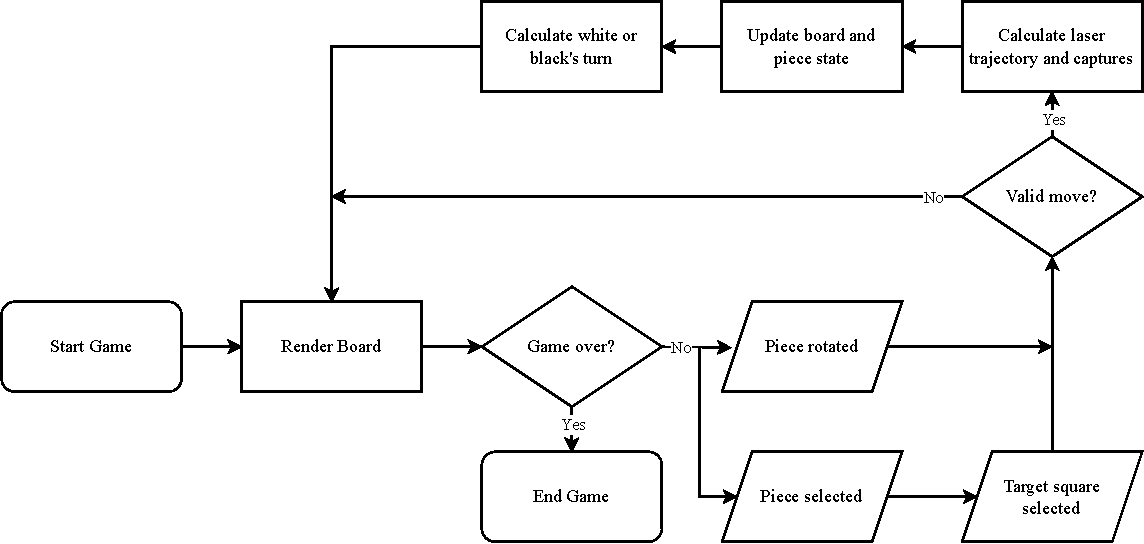
\includegraphics[width=\columnwidth]{../design/assets/game_flowchart.pdf}
    \caption{Flowchart for Game}
    \label{fig:game-flowchart}
\end{figure}

\subsubsection{Board Editor}
\begin{figure}[ht!]
    \centering
    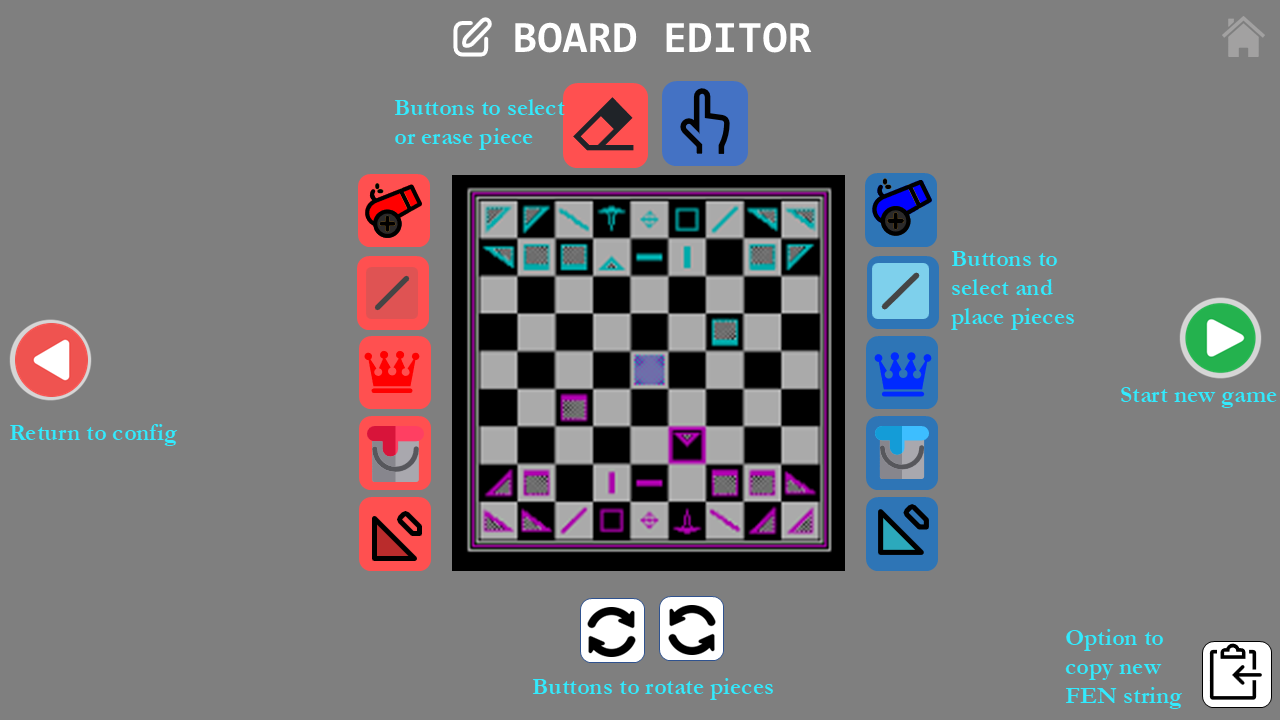
\includegraphics[width=0.8\columnwidth]{../design/assets/editor_gui.png}
    \caption{Editor screen prototype}
    \label{fig:editor-gui}
\end{figure}

The editor screen is used to configure the starting position of the board. Controls should include the ability to place all piece types of either colour, to erase pieces, and easy board manipulation shortcuts such as dragging pieces or emptying the board.

For the GUI, the buttons should clearly represent their functionality, through the use of icons and appropiate colouring (e.g. red for delete).

\begin{figure}[ht!]
    \centering
    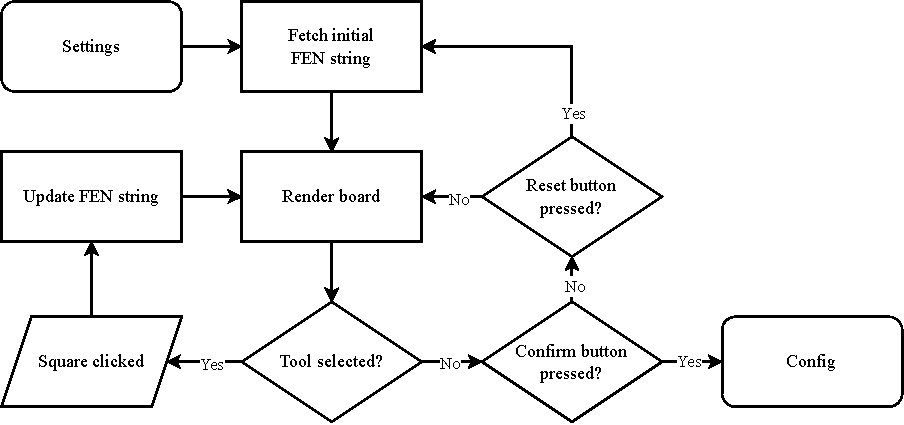
\includegraphics[width=\columnwidth]{../design/assets/editor_flowchart.pdf}
    \caption{Flowchart for board editor}
    \label{fig:editor-flowchart}
\end{figure}

\subsection{Algorithms and Techniques}
\subsubsection{Minimax}
Minimax is a backtracking algorithm commonly used in zero-sum games used to determine the score according to an evaluation function, after a certain number of perfect moves. Minimax aims to minimize the maximum advantage possible for the opponent, thereby minimizing a player’s possible loss in a worst-case scenario. It is implemented using recursive depth-first search, alternating between minimizing and maximizing the player’s advantage in each recursive call.

\begin{figure}[ht!]
    \centering
    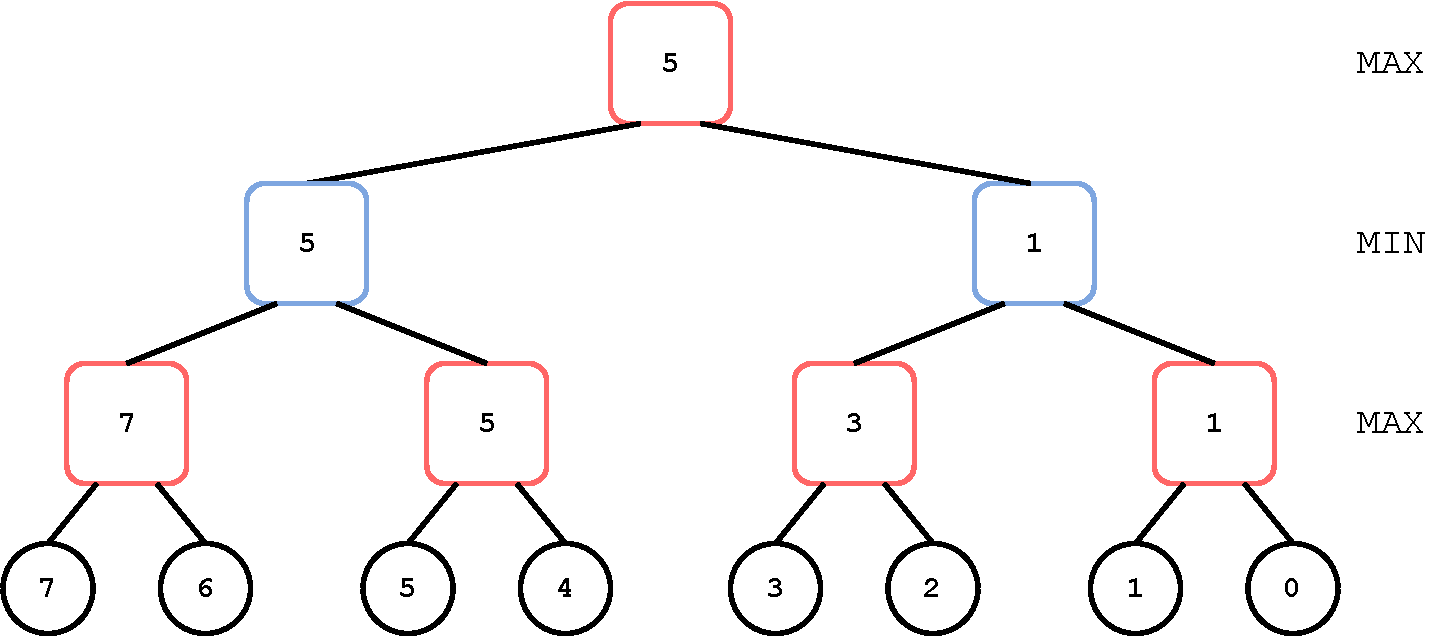
\includegraphics[width=\columnwidth]{../design/assets/minimax.pdf}
    \caption{Example minimax tree}
    \label{fig:minimax}
\end{figure}

For the example minimax tree show in Figure \ref{fig:minimax}, starting from the bottom leaf node evaluations, the maximizing player would choose the highest values (7, 5, 3, 1). From those values, the minimizing player would choose the lowest values (5, 1). The final value chosen by the maximum player would therefore be the highest of the two, 5.

\noindent Implementation in the form of pseudocode is shown below:

\begin{algorithm}
\caption{Minimax pseudocode}
\begin{algorithmic}
    \Function{minimax}{node, depth, maximizingPlayer}
        \If{$depth = 0$ \textbf{OR} node equals game over}
            \State \Return{\Call{evaluate}{}}
        \EndIf
        
        \bigskip

        \If{maximisingPlayer}
            \State $value \gets -\infty$
            \For{child of node}
                \State $value \gets \Call{max}{value, \Call{minimax}{child, depth - 1, false}}$
            \EndFor
            \State \Return{$value$}
        \Else
            \State $value \gets +\infty$
            \For{child of node}
                \State $value \gets \Call{min}{value, \Call{minimax}{child, depth - 1, true}}$
            \EndFor
            \State \Return{$value$}
        \EndIf
    \EndFunction
\end{algorithmic}
\end{algorithm}

\subsubsection{Minimax improvements}
\subsubsection*{Alpha-beta pruning}
Alpha-beta pruning is a search algorithm that aims to decrease the number of nodes evaluated by the minimax algorithm. Alpha-beta pruning stops evaluating a move in the game tree when one refutation is found in its child nodes, proving the node to be worse than previously-examined alternatives. It does this without any potential of pruning away a better move.
The algorithm maintains two values: alpha and beta. Alpha ($\alpha$), the upper bound, is the highest value that the maximizing player is guaranteed of; Beta ($\beta$), the lower bound, is the lowest value that the minimizing player is guaranteed of. If the condition $\alpha\geq\beta$ for a node being evaluated, the evaluation process halts and its remaining children nodes are ‘pruned’.

\noindent This is shown in the following maximizing example:  

\begin{figure}[ht!]
    \centering
    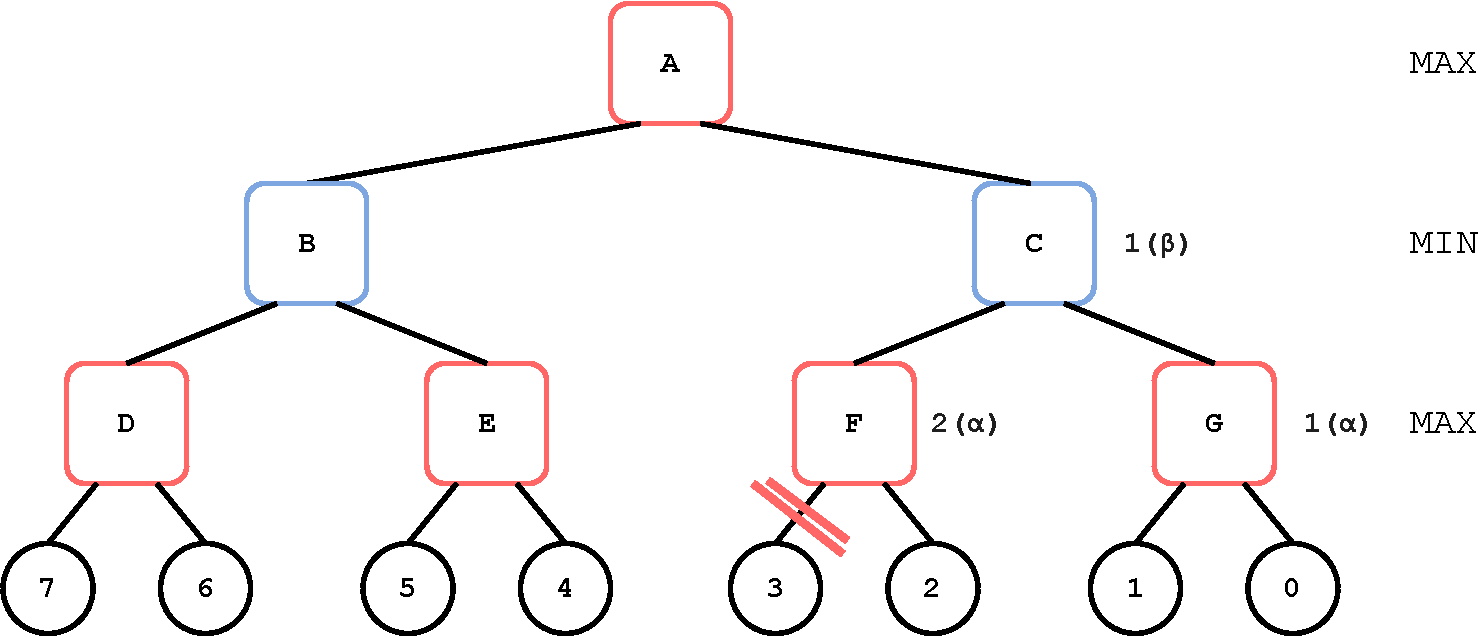
\includegraphics[width=\columnwidth]{../design/assets/alpha_beta_pruning.pdf}
    \caption{Example minimax tree with alpha-beta pruning}
    \label{fig:alpha-beta}
\end{figure}

Since minimax is a depth-first search algorithm, nodes $C$ and $G$ and their $\alpha$ and $\beta$ have already been searched. Next, at node $F$, the current $\alpha$ and $\beta$ are $-\infty$ and 1 respectively, since the $\beta$ is passed down from node $C$. Searching the first leaf node, the $\alpha$ subsequently becomes $\alpha=max(-\infty,2)$. This means that the maximising player at this depth is already guaranteed an evaluation of 2 or greater. Since we know that the minimising player at the depth above is guaranteed a value of 1, there is no point in continuing to search node $F$, a node that is returns a value of 2 or greater. Hence at node $F$, where $\alpha\geq\beta$, the branches are pruned.

Alpha-beta pruning therefore prunes insignificant nodes by maintain an upper bound $\alpha$ and lower bound $\beta$. This is an essential optimization as a simple minimax tree increases exponentially in size with each depth ($O(b^d)$, with branching factor $b$ and $d$ ply depth), and alpha-beta reduces this and the associated computational time considerably.

\noindent The pseudocode implementation is shown below:

\begin{algorithm}
\caption{Minimax with alpha-beta pruning pseudocode}
\begin{algorithmic}
    \Function{minimax}{node, depth, $\alpha$, $\beta$, maximizingPlayer}
        \If{$depth = 0$ \textbf{OR} node equals game over}
            \State \Return{\Call{evaluate}{}}
        \EndIf

        \bigskip

        \If{maximisingPlayer}
            \State $value \gets -\infty$
            \For{child of node}
                \State $value \gets \Call{max}{value, \Call{minimax}{child, depth - 1, \alpha, \beta, false}}$
                \If{$value > \beta$}
                    \textbf{break}
                \EndIf
                \State $\alpha \gets \Call{max}{\alpha, value}$
            \EndFor
            \State \Return{$value$}
        \Else
            \State $value \gets +\infty$
            \For{child of node}
                \State $value \gets \Call{min}{value, \Call{minimax}{child, depth - 1, \alpha, \beta, true}}$
                \If{$value < \alpha$}
                    \textbf{break}
                \EndIf
                \State $\beta \gets \Call{min}{\beta, value}$
            \EndFor
            \State \Return{$value$}
        \EndIf
    \EndFunction
\end{algorithmic}
\end{algorithm}

\subsubsection*{Transposition Tables \& Zobrist Hashing}
Transition tables, a  memoisation technique, again greatly reduces the number of moves searched. During a brute-force minimax search with a depth greater than 1, the same positions may be searched multiple times, as the same position can be reached from different sequences of moves. A transposition table caches these same positions (transpositions), along with the its associated evaluations, meaning commonly reached positions are not unnecessarily re-searched.

Flags and depth are also stored alongside the evaluation. Depth is required as if the current search comes across a cached position with an evaluation calculated at a lower depth than the current search, the evaluation may be inaccurate. Flags are required for dealing with the uncertainty involved with alpha-beta pruning, and can be any of the following three.

\paragraph{Exact} flag is used when a node is fully searched without pruning, and the stored and fetched evaluation is accurate.
\paragraph{Lower} flag is stored when a node receives an evaluation greater than the $\beta$, and is subsequently pruned, meaning that the true evaluation could be higher than the value stored. We are thus storing the $\alpha$ and not an exact value. Thus, when we fetch the cached value, we have to recheck if this value is greater than $\beta$. If so, we return the value and this branch is pruned (fail high); If not, nothing is returned, and the exact evaluation is calculated.
\paragraph{Upper} flag is stored when a node receives an evaluation smaller than the $\alpha$, and is subsequently pruned, meaning that the true evaluation could be lower than the value stored. Similarly, when we fetch the cached value, we have to recheck if this value is lower than $\alpha$. Again, the current branch is pruned if so (fail low), and an exact evaluation is calculated if not.

\noindent The pseudocode implementation for transposition tables is shown below:

\begin{algorithm}
\caption{Minimax with transposition table pseudocode}
\begin{algorithmic}
    \Function{minimax}{node, depth, $\alpha$, $\beta$, maximizingPlayer}
        \State $hash\_key \gets \Call{hash}{node}$
        \State $entry \gets \Call{getentry}{hash\_key}$

        \bigskip

        \If{$entry.hash\_key = hash\_key$ \textbf{AND} $entry.hash\_key \geq depth$}
            \If{$entry.hash\_key = \textbf{EXACT}$}
                \State \Return{$entry.value$}
            \ElsIf{$entry.hash\_key = \textbf{LOWER}$}
                \State $\alpha \gets \Call{max}{\alpha, entry.value}$

            \ElsIf{$entry.hash\_key = \textbf{UPPER}$}
                \State $\beta \gets \Call{min}{\beta, entry.value}$
            \EndIf

            \If{$\alpha\geq\beta$}
                \State \Return{$entry.value$}
            \EndIf
        \EndIf

        \bigskip

        \textit{...normal minimax...}

        \bigskip

        \State $entry.value \gets value$
        \State $entry.depth \gets depth$
        \If{$value \leq \alpha$}
            \State $entry.flag \gets \textbf{UPPER}$
        \ElsIf{$value \geq \beta$}
            \State $entry.flag \gets \textbf{LOWER}$
        \Else
            \State $entry.flag \gets \textbf{EXACT}$
        \EndIf

        \bigskip

        \Return{$value$}
    \EndFunction
\end{algorithmic}
\end{algorithm}

The current board position will be used as the index for a transposition table entry. To convert our board state and bitboards into a valid index, Zobrist hashing may be used. For every square on the chessboard, a random integer is assigned to every piece type (12 in our case, 6 piece type, times 2 for both colours). To initialise a hash, the random integer associated with the piece on a specific square undergoes a XOR operation with the existing hash. The hash is incrementally update with XOR operations every move, instead of being recalculated from scratch improving computational efficiency. Using XOR operations also allows moves to be reversed, proving useful for the functionality to scroll throughh previous moves. A Zobrist hash is also a better candidate than FEN strings in checking for threefold-repetition, as they are less intensive to calculate for every move.

\noindent The pseudocode implementation for Zobrist hashing is shown below:

\begin{algorithm}
\caption{Zobrist hashing pseudocode}
\begin{algorithmic}
    \item \textit{RANDOMINTS represents a pre-initialised array of random integers for each piece type for each square}
    
    \bigskip

    \Function{hashboard}{board}
        \State $hash \gets 0$

        \For{each square on board}
            \If{square is not empty}
                \State $hash \oplus RANDOMINTS[square][$\textit{piece on square}$]$
            \EndIf
        \EndFor
        
        \State \Return $hash$
    \EndFunction

    \bigskip

    \Function{updatehash}{hash, move}
        \State $hash \oplus RANDOMINTS[$\textit{source square}$][$\textit{piece}$]$
        \State $hash \oplus RANDOMINTS[$\textit{destination square}$][$\textit{piece}$]$

        \If{red to move}
            \State $hash \oplus \textit{hash for red to move}$ \Comment{Hash needed for move colour, as two identical positions are different if the colour to move is different}
        \EndIf
        
        \State \Return $hash$
    \EndFunction
\end{algorithmic}
\end{algorithm}




\subsection{Classes}
\end{document}